\section{\absmachine: An abstract machine for programmable switches}
\label{s:absmachine}

% TODO: Say that the atoms can't write to the same packet field.
Having described the compiler frontend, we now formally describe the abstract
machine, \textit{\absmachine}, the compiler target for \pktlanguage before
describing the compiler backend.  \absmachine captures several important
features of programmable switch architectures~(\S\ref{ss:abstract}) with
deterministic performance.

\begin{figure*}[!t]
  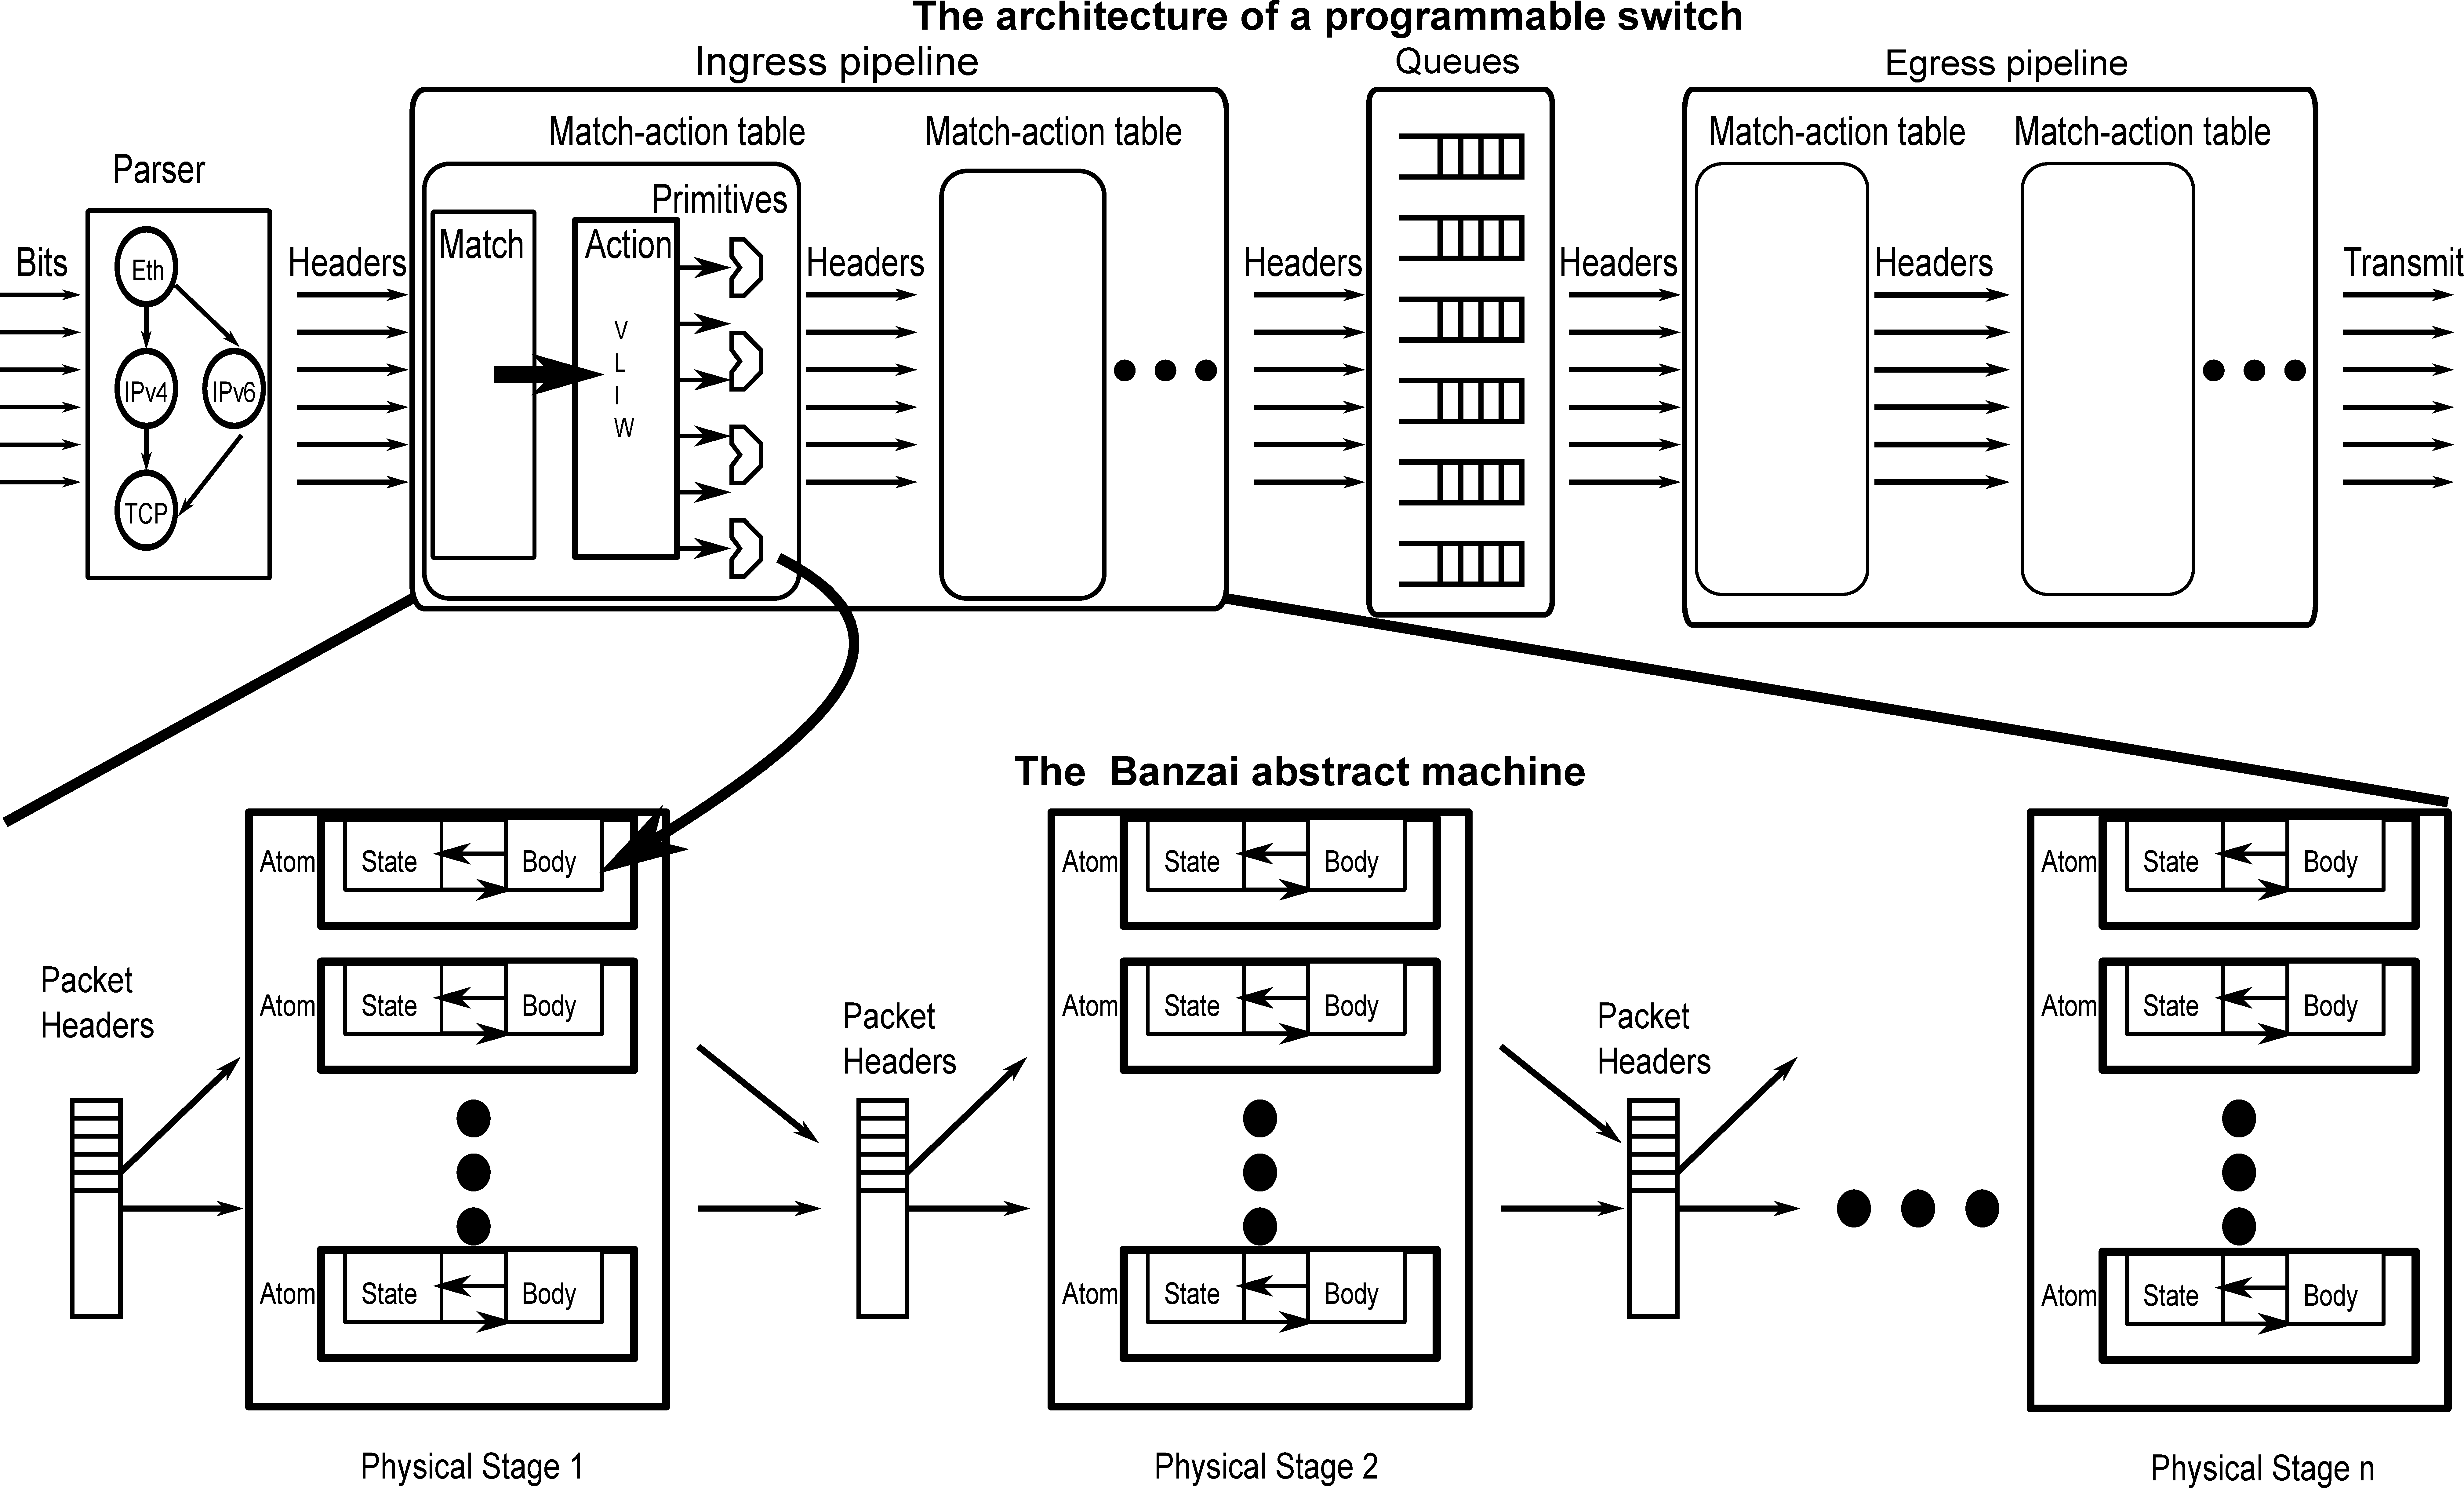
\includegraphics[width=\textwidth]{banzai.pdf}
  \caption{The \absmachine abstract machine and its relationship to programmable switch architectures.}
  \label{fig:switch}
\end{figure*}
Our abstract machine is directly inspired by programmable switch architectures
such as the Reconfigurable Match-Action Table architecture (RMT), Intel's
FlexPipe architecture, and Cavium's XPliant architecture. These architectures
assume a switch model (Figure~\ref{fig:switch}) that consists of an ingress
pipeline, followed by the switch scheduler, followed by an egress pipeline.

\absmachine is an abstract machine that models either of these two pipelines,
with the only difference being the packet fields available at the entrance of
these pipelines. Being an abstract machine, \absmachine only models mechanisms
that are critical to mapping data-plane algorithms. In particular, it models
the computation that happens in each match-action table (i.e. the action half
of the match-action table), but not the match semantics (direct, ternary, or
longest prefix). Notably, \absmachine doesn't model packet parsing, assuming
that packets are handed to it already parsed.

A switch pipeline in \absmachine has a number of pipeline stages that execute
synchronously on every time step. Further, every pipeline stage is assumed to
have the latency of one time step. Once a pipeline stage processes a packet, it
hands it off to the next pipeline stage.  Each stage contains a vector of
\textit{atoms}, with the atoms executing in parallel.

Informally, an atom is an atomic unit of packet processing and is represented
by a body of imperative code that executes sequentially. An atom is assumed to
complete execution and modify a packet before the next packet is processed by
that atom. Atoms within a stage may modify any packet field so long as two
atoms in a stage do not modify the same packet field.

An atom may also contain internal state that can influence the atom's behavior
from one packet to the next and persists across packets. For instance, a switch
counter could be written as an atom as follows\footnote{We use the notation p.x
to represent access to field ``x'' within a packet p and the notation x to
represent access to the state variable ``x'' that persists across packets}.
\begin{verbatim}
  p.tmp     = counter;
  p.tmp2    = p.tmp + 1;
  counter   = p.tmp2;
\end{verbatim}
Similarly, a stateless operation that sets a packet field, such as the
modify\_field action primitive in P4 (equivalently, the bitmasked-set operation
from the RMT architecture) can be written as the atom below:
\begin{verbatim}
  p.field   = value;
\end{verbatim}

The \absmachine abstract machine generalizes several aspects of programmable
switch architectures. The vector of atoms in each stage generalizes RMT's
very-large instruction-word (VLIW)~\cite{rmt} that executes primitive actions
on independent packet fields in parallel. The presence of internal state in an
atom models persistent switch state residing on a switch such as meters,
counters, and P4's register abstraction in a unified manner.

\subsection{Constraints on atoms}

To run at line rate, we will need to constrain the behavior of atoms to provide
deterministic performance. We impose two such constraints that distinguish
\absmachine from software routers such as Click and Network Processors such as
the Intel IXP, which tradeoff deterministic performance for increased
programmability.

First, \absmachine is a shared-nothing machine: state variables are internal to
a particular atom and their values can only be communicated with atoms in
subsequent stages by writing them into packet fields that are then read
downstream.  This restriction reflects the capabilities of most switches today:
simultaneously accessing memory from multiple switch stages is technically
challenging because it requires building power-hungry multi-ported RAMs.

Second, we constrain the complexity of atom bodies by definining how atoms are
executed. One execution model is an in-order CPU that can execute at most $N$
instructions sequentially. Another is a configurable combinational circuit in
hardware~\cite{dataflow}, where the space of control signals to the circuit
limits the space of feasible computations within the atom. These two execution
models are by no means exhaustive: as programmable switches evolve, we expect
the computational capabilities of atoms to evolve as well.

\subsection{Parametrizing \absmachine}

A \absmachine abstract machine has three parameters:
\begin{enumerate}
\item The number of pipeline stages, which correspond to the number of physical stages
  in a programmable switch.
\item A limit on the number of concurrent atoms in a pipeline stage, which corresponds
  to the width of the VLIW used to execute actions on a packet header.
\item Constraints on atoms themselves, which models limits on the amount of useful
  computation that can happen in an atom while still maintaining line rate.
\end{enumerate}
In our evaluations, we instantiate \absmachine with several parameter settings
that correspond to natural constraints on switch architectures. We then
evaluate how different instantiations of \absmachine affect the
implementability of several data-plane algorithms.

% TODO: Move this to evaluation.
% We use both models in this paper. For stateless atoms that don't modify state,
% we constrain atom bodies to consist of only statements that can be represented
% as three-instruction codes. Further, we allow exactly one statement in each
% atom body. This corresponds to the set of primitive actions available today in
% P4/RMT.  For atoms that do modify state, we consider both models
% (\S\ref{s:constraints}) and evaluate how atom body constraints affect whether
% or not packet-processing code can be mapped onto \absmachine.
